\documentclass[a4paper,12pt,twoside,openright,titlepage]{book}

%Additional packages
\usepackage[utf8]{inputenc}
\usepackage[T1]{fontenc}
\usepackage[dutch,english]{babel}
\usepackage{imakeidx}
\usepackage{syntonly}
\usepackage[official]{eurosym}
%\usepackage[graphicx]
\usepackage{graphicx}
\graphicspath{ {./images/} }
\usepackage{float}
\usepackage{xurl}
\usepackage{hyperref}
\hypersetup{colorlinks=true, linkcolor=blue, citecolor=blue, filecolor=blue, urlcolor=blue, pdftitle=, pdfauthor=, pdfsubject=, pdfkeywords=}
\usepackage{tabularx}
\usepackage[table]{xcolor} % Table colors
\usepackage{scrextend}
\addtokomafont{labelinglabel}{\sffamily}
\usepackage{listings}
\usepackage{adjustbox}
\usepackage{color}

% Define colors
\definecolor{ashgrey}{rgb}{0.7, 0.75, 0.71}

% Listing style
\lstset{
  backgroundcolor=\color{ashgrey}, % choose the background color; you must add \usepackage{color} or \usepackage{xcolor}; should come as last argument
  basicstyle=\footnotesize,        % the size of the fonts that are used for the code
  breakatwhitespace=true,          % sets if automatic breaks should only happen at whitespace
  breaklines=true,                 % sets automatic line breaking
  extendedchars=true,              % lets you use non-ASCII characters; for 8-bits encodings only, does not work with UTF-8
  frame=single,	                   % adds a frame around the code
  rulecolor=\color{black},         % if not set, the frame-color may be changed on line-breaks within not-black text (e.g. comments (green here))
  keepspaces=true,                 % keeps spaces in text, useful for keeping indentation of code (possibly needs columns=flexible)
  columns=fullflexible,		   % make copy and paste possible
  showstringspaces=false,          % if true show spaces in strings adding particular underscores
  showspaces=false,                % if true show spaces everywhere adding particular underscores; it does not override 'showstringspaces'
}

% Uncomment for production
% \syntaxonly

% Style
\pagestyle{headings}

% Turn on indexing
\makeindex[intoc]

% Define document
\author{D. Leeuw}
\title{Boolean Algebra}
\date{\today\\v.1.1.0}

\begin{document}
\selectlanguage{dutch}

\maketitle

\copyright\ 2023 Dennis Leeuw\\

\begin{figure}

\includegraphics[width=0.3\textwidth]{CC-BY-SA-NC.png}
\end{figure}

\bigskip

Dit werk is uitgegeven onder de Creative Commons BY-NC-SA Licentie en laat anderen toe het werk te kopi\"eren, distribueren, vertonen, op te voeren, en om afgeleid materiaal te maken, zolang de auteurs en uitgever worden vermeld als maker van het werk, het werk niet commercieel gebruikt wordt en afgeleide werken onder identieke voorwaarden worden verspreid.


%%%%%%%%%%%%%%%%%%%
%%% Introductie %%%
%%%%%%%%%%%%%%%%%%%

\frontmatter
\chapter{Over dit Document}
\section{Leerdoelen}
Dit document geeft een basis uitleg over de boolean algebra in relatie tot de elektrotechniek. De verschillende Boolean functies worden beschreven aan de hand van elektronische schema's. De lezer leert dan ook wat boolean algebra is in de context van de elektrotechniek.


\section{Voorkennis}
\begin{itemize}
\item Om de uitleg te kunnen volgen die beschreven is bij de elektronische werking van de verschillende functies dient de lezer kennis te hebben van de werking van transistoren, weerstanden, spanning en stroom
\item Het is handig als de lezer enigzins vertrouwd is met het lezen van stroomschema's
\end{itemize}


%%%%%%%%%%%%%%%%%
%%% De inhoud %%%
%%%%%%%%%%%%%%%%%
\tableofcontents

\mainmatter

\chapter{Introduction}
In dit hoofdstuk gaan we een aantal van de hiervoor beschreven componenten gebruiken gebruiken om computer logica op te bouwen. Kortom hoe maken we van elektrische spanningen logische circuits. De booleanse algebra\index{Booleanse algebra}, een tak van de wiskunde, onderscheidt zich van de rest van de wiskunde doordat de booleanse algebra alleen gebruik maakt van true of false, of zoals we in de computer techniek zeggen 1 en 0.

In de computertechniek gebruiken we de transistor als schakelaar. De basis van de transistor is de input. Door deze input te gebruiken schakelen we de transistor en komt er een bepaalde waarde (1 of 0) aan de output.

De gebruikte spanningen in de computer zijn 3,3 Vdc of 5 Vdc en dat is dan een 1. De 0 is staat gelijk aan geen spanning.

De booleanse algebra wordt ook gebruikt bij het programmeren van computers. Dan staan de waarden 1 of 0 vaak voor true of false. Een vergelijking is waar of niet waar. We zullen hier niet al te doen op ingaan. Wel belangrijk is het om te weten dat je een 1 dus kan lezen als waar en een 0 als niet waar.



\chapter{NOT - Inverter}
De NOT\index{NOT} werkt als een inverter\index{Inverter}. Dus als er een 1 op de ingang wordt aangeboden dan staat er een 0 op de uitgang en omgekeerd. De waarheidstabel voor de inverter is dus heel eenvoudig:


De NOT wordt gebouwd door gebruik van een enkele transistor en een weerstand (figuur \ref{circuit:not}.

\begin{figure}[h]
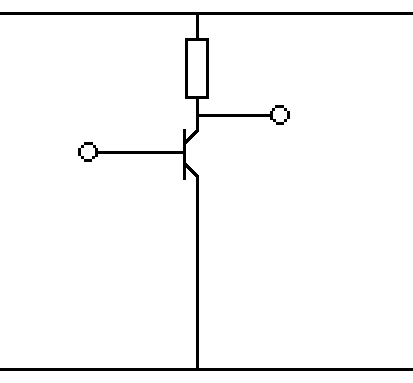
\includegraphics{inverter_circuit}
\centering
\caption{NOT circuit}
\label{circuit:not}
\end{figure}



\rowcolors{2}{gray!10}{gray!20}
\begin{tabular}{ |c|c| }
\hline
\rowcolor{gray!60}
Input & Output \\
\hline
0 & 1 \\
\hline
1 & 0 \\
\hline
\end{tabular}


Het symbool voor de NOT is weergegeven in figuur \ref{symbool:not}

\begin{figure}[h]
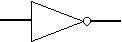
\includegraphics{inverter_symbool}
\centering
\caption{Symbool van een NOT}
\label{symbool:not}
\end{figure}


In de wiskunde of in programmeertalen kan je de not tegenkomen met de volgende symbolen:
\begin{math}
\lnot \; !
\end{math}



\chapter{AND}
De AND\index{AND} geeft aan dat wanneer beide waarden 1 zijn ook de uitkomst 1 is.


De AND wordt gebouwd door gebruik te maken van twee transistoren waarvan de beide basis de ingang vormen en een weerstand (figuur \ref{circuit:and}.

\begin{figure}[h]
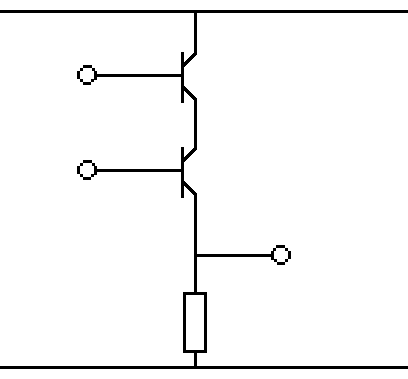
\includegraphics{and_circuit}
\centering
\caption{AND circuit}
\label{circuit:and}
\end{figure}


\rowcolors{2}{gray!10}{gray!20}
\begin{tabular}{ |c|c|c| }
\hline
\rowcolor{gray!60}
	Input 1 & Input 2 & Output \\
	\hline
	0 & 0 & 0 \\
	\hline
	0 & 1 & 0 \\
	\hline
	1 & 0 & 0 \\
	\hline
	1 & 1 & 1 \\
	\hline
\end{tabular}


Het symbool in een stroomschema voor de AND is weergegeven in figuur \ref{symbool:and}

\begin{figure}[h]
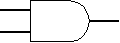
\includegraphics{and_symbool}
\centering
\caption{Symbool van een AND}
\label{symbool:and}
\end{figure}


In wiskundige notaties en bij het programeren kunnen de volgende symbolen gebruikt worden om een AND aan te geven (afhankelijk van de programeertaal):
\begin{math}
\land \; \& \; \&\& \; \cdot
\end{math}



\chapter{NAND}
De NAND\index{NAND} geeft een negatief resultaat als beide ingangen 1 zijn, de uitgang is dan 0.

De NAND-technologie kan je tegen komen in flash memory.



De NAND wordt gebouwd door gebruik te maken van twee transistoren waarvan de beide basis de ingang vormen en een weerstand (figuur \ref{circuit:nand}.

\begin{figure}[h]
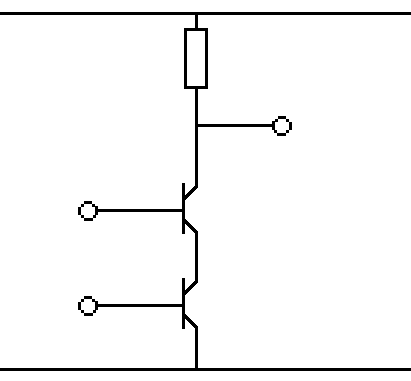
\includegraphics{nand_circuit}
\centering
\caption{NAND circuit}
\label{circuit:nand}
\end{figure}



\rowcolors{2}{gray!10}{gray!20}
\begin{tabular}{ |c|c|c| }
\hline
\rowcolor{gray!60}
	Input 1 & Input 2 & Output \\
	\hline
	0 & 0 & 1 \\
	\hline
	0 & 1 & 1 \\
	\hline
	1 & 0 & 1 \\
	\hline
	1 & 1 & 0 \\
	\hline
\end{tabular}


Het symbool voor de NAND is weergegeven in figuur \ref{symbool:nand}

\begin{figure}[h]
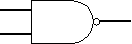
\includegraphics{nand_symbool}
\centering
\caption{Symbool van een NAND}
\label{symbool:nand}
\end{figure}


\input{src/nand-prog}

\chapter{OR}
De OR\index{OR} geeft aan of \'e\'en of beide ingangen 1 zijn, als dat het geval is dan is de uitgang 1.


De OR wordt gebouwd door gebruik te maken van twee transistoren die parallel aan elkaar staan, de beide basis vormen de ingang en er is een weerstand (figuur \ref{circuit:or}.

\begin{figure}[h]
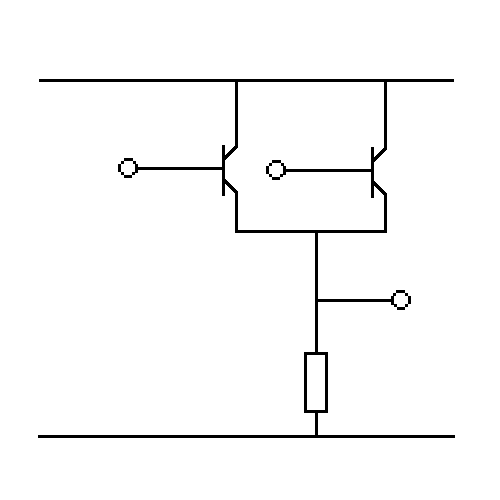
\includegraphics{or_circuit}
\centering
\caption{OR circuit}
\label{circuit:or}
\end{figure}



\rowcolors{2}{gray!10}{gray!20}
\begin{tabular}{ |c|c|c| }
\hline
\rowcolor{gray!60}
	Input 1 & Input 2 & Output \\
	\hline
	0 & 0 & 0 \\
	\hline
	0 & 1 & 1 \\
	\hline
	1 & 0 & 1 \\
	\hline
	1 & 1 & 1 \\
	\hline
\end{tabular}


Het symbool voor de OR is weergegeven in figuur \ref{symbool:or}

\begin{figure}[h]
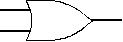
\includegraphics{or_symbool}
\centering
\caption{Symbool van een OR}
\label{symbool:or}
\end{figure}


In de wiskunde of in programmeertalen kan je de OR tegen komen met de volgende symbolen:
\begin{math}
\lor \; \parallel
\end{math}



\chapter{NOR}
De NOR\index{NOR} geeft aan dat beide ingangen 0 zijn, als dat het geval is dan is de uitgang 1.

De NOR-technologie kan je tegen komen in flash memory.


De NOR wordt gebouwd door gebruik te maken van twee transistoren die parallel aan elkaar staan, de beide basis vormen de ingang en er is een weerstand (figuur \ref{circuit:nor}.

\begin{figure}[h]
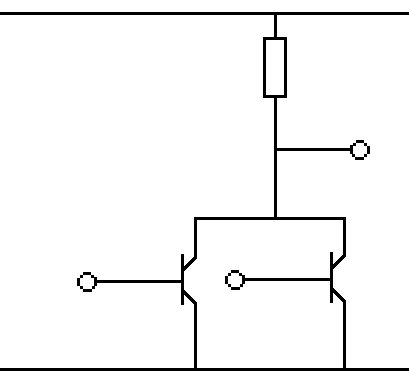
\includegraphics{nor_circuit}
\centering
\caption{NOR circuit}
\label{circuit:nor}
\end{figure}



\rowcolors{2}{gray!10}{gray!20}
\begin{tabular}{ |c|c|c| }
\hline
\rowcolor{gray!60}
	Input 1 & Input 2 & Output \\
	\hline
	0 & 0 & 1 \\
	\hline
	0 & 1 & 0 \\
	\hline
	1 & 0 & 0 \\
	\hline
	1 & 1 & 0 \\
	\hline
\end{tabular}


Het symbool voor de NOR is weergegeven in figuur \ref{symbool:nor}

\begin{figure}[h]
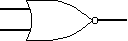
\includegraphics{nor_symbool}
\centering
\caption{Symbool van een NOR}
\label{symbool:nor}
\end{figure}


\input{src/nor-prog}

\chapter{XOR}
De XOR\index{XOR} geeft alleen als \'e\'en van beide ingangen 1 is een 1 op de uitgang. De XOR functie wordt veel gebruikt in de cryptografie\index{Cryptografie}.


Er zijn vele manieren om een XOR te bouwen, er is dan ook geen circuit opgenomen. Zie Wikipedia voor mogelijke oplossingen.



\rowcolors{2}{gray!10}{gray!20}
\begin{tabular}{ |c|c|c| }
\hline
\rowcolor{gray!60}
	Input 1 & Input 2 & Output \\
	\hline
	0 & 0 & 0 \\
	\hline
	0 & 1 & 1 \\
	\hline
	1 & 0 & 1 \\
	\hline
	1 & 1 & 0 \\
	\hline
\end{tabular}


Het symbool voor de XOR is weergegeven in figuur \ref{symbool:xor}

\begin{figure}[h]
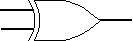
\includegraphics{xor_symbool}
\centering
\caption{Symbool van een XOR}
\label{symbool:xor}
\end{figure}


In de wiskunde of in programmeertalen kan je de XOR tegenkomen met de volgende symbolen:
\begin{math}
\oplus \; 
\end{math}



\chapter{XNOR}
De XNOR\index{XNOR} geeft als \'e\'en van beide ingangen 1 is en de andere 0 een 0 op de uitgang.


Er zijn vele manieren om een XNOR te bouwen, er is dan ook geen circuit opgenomen. Zie Wikipedia voor mogelijke oplossingen.



\rowcolors{2}{gray!10}{gray!20}
\begin{tabular}{ |c|c|c| }
\hline
\rowcolor{gray!60}
	Input 1 & Input 2 & Output \\
	\hline
	0 & 0 & 1 \\
	\hline
	0 & 1 & 0 \\
	\hline
	1 & 0 & 0 \\
	\hline
	1 & 1 & 1 \\
	\hline
\end{tabular}


Het symbool voor de XNOR is weergegeven in figuur \ref{symbool:xnor}

\begin{figure}[h]
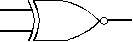
\includegraphics{xnor_symbool}
\centering
\caption{Symbool van een XNOR}
\label{symbool:xnor}
\end{figure}


\input{src/xnor-prog}

\chapter{Praktijkopdrachten}
Met een breadboard kunnen de verschillende boolean functies nagebouwd worden. Sluit op de uitgang van de transistor een weerstand en een led aan en kies voor de basis van elke transistor een juiste weerstand en spanning om een 1 aan te kunnen bieden.



%%%%%%%%%%%%%%%%%%%%%
%%% Index and End %%%
%%%%%%%%%%%%%%%%%%%%%
\backmatter
\printindex
\end{document}

%%% Last line %%%
